%%%%%%%%%%%%%%%%%%%%%%%%%%%%%%%%%%%%%%%%%%%%%%%%%%%%%%%%%%%%%%%%%%%%%%%
% Ansys Techcon 2022 - API Guidance and Best Practices
%%%%%%%%%%%%%%%%%%%%%%%%%%%%%%%%%%%%%%%%%%%%%%%%%%%%%%%%%%%%%%%%%%%%%%%
\documentclass[t]{beamer}

\usetheme{Ansys2022}

\usepackage{bbding,pifont}
\usepackage{minted}
\usepackage{xcolor}
\usepackage{pdfpages}
\usepackage{listings}
\usepackage{hyperref}

\usepackage{tikz}
\usetikzlibrary{intersections}
\usetikzlibrary{shapes.geometric, arrows,positioning}

\usepackage[edges]{forest}
\hypersetup{
    colorlinks=true,
    linkcolor=blue,
    filecolor=magenta,      
    urlcolor=cyan,
}
 

\urlstyle{same}
\setbeamercolor{background canvas}{bg=}

\definecolor{bleudefrance}{rgb}{0.19, 0.55, 0.91}

%%%%%%%%%%%%%%%%%%%%%%%%%%%%%%%%%%%%%%%%%%%%%%%%%%%%%%%%%%%%%%%%%%%%%%%%%%%%%%%

\tikzset{
  startstop/.style={
    rectangle, 
    rounded corners,
    minimum width=3cm,
    minimum height=0.75cm,
    align=center, 
    draw=black, 
    fill=ANSYS@Gold,
    },
  process/.style={
    rectangle, 
    minimum width=3cm, 
    minimum height=0.75cm, 
    align=center, 
    draw=black, 
    fill=ANSYS@Blue,
    text=white,
    },
  decision/.style={
    diamond, 
    aspect=4,
    minimum width=3cm, 
    minimum height=1cm,
    align=center,
    draw=black, 
    fill=ANSYS@Blue,
    text=white,
    },
  arrow/.style={thick,->,>=stealth},
  dec/.style={
    ellipse, 
    align=center, 
    draw=black, 
    fill=ANSYS@Bronze,
    },
}

\begin{document}

%%%%%%%%%%%%%%%%%%%%%%%%%%%%%%%%%%%%%%%%%%%%%%%%%%%%%%%%%%%%%%%%%%%%%%%%%%%%%%%
%% Title Slide

\title{API Guidance and Best Practices}
%% \subtitle{}
\author{Alex Kaszyski \\ Roberto Pastor Muela}
\date{\today}

\titleframe{}


%%%%%%%%%%%%%%%%%%%%%%%%%%%%%%%%%%%%%%%%%%%%%%%%%%%%%%%%%%%%%%%%%%%%%%%%%%%%%%%
%% Table of contents

\begin{frame}{Table of Contents}
  \tableofcontents
  \vspace{200pt}  %% force top tight  
\end{frame}


%%%%%%%%%%%%%%%%%%%%%%%%%%%%%%%%%%%%%%%%%%%%%%%%%%%%%%%%%%%%%%%%%%%%%%%%%%%%%%%
\section{Why APIs? - Problem Definition}
\begin{frame}
  \frametitle{APIs - Problem Space}

  \begin{columns}[T]
    \begin{column}{.6\textwidth}

      %% The duration of this talk could easily be for a couple of hours, but
      %% since we only have 15 minutes, let's try to narrow the solution space to
      %% APIs and customer needs.

      \textbf{What do customers want?} Let's consider two kinds of customers
      who might want APIs:

      \begin{itemize}
      \item{Those who want to automate repetitive workflows.}
      \item{Those who need low-level access to the underlying libraries and
        components that make up an Ansys product.}
      \end{itemize}

      %% Companies used to spend a huge part of their resources in employees
      %% manually configuring and running simulations. Nowadays, most customers
      %% want to automate this process, such that by easily modifying an
      %% automated script they can rerun their simulations and evaluate the
      %% impact of these changes.

      %% Automation is a key point - having a person "behind the wheel" is
      %% sometimes necessary but once you have proven that your automation
      %% tools work, they are less error prone.

      \textbf{What do developers want?}
      
      \begin{itemize}
      \item{Well documented low-level interface to foreign libraries to avoid
        duplicating work.}
      \end{itemize}

      %% Developers use APIs all the time. These are the public interfaces that
      %% enable other developers to use their libraries.

    \end{column}

    \begin{column}{.45\textwidth}
      %% \centering
      \def\firstcircle{(0,0) circle (1.75cm)}
      \def\secondcircle{(60:2cm) circle (1.75cm)}
      \def\thirdcircle{(0:2cm) circle (1.75cm)}
      \begin{tikzpicture}
        \begin{scope}[shift={(3cm,-5cm)}, fill opacity=0.75]
          \fill[gray] \firstcircle;
          \fill[ANSYS@Bronze] \secondcircle;
          \fill[ANSYS@Blue] \thirdcircle;
          \draw \firstcircle node[below,text width=4cm,align=center,shift={(-2ex,0ex)}] {\footnotesize Product\\ Automation};
          \draw \secondcircle node [above,text width=4cm,align=center,shift={(0ex,2ex)}] {\footnotesize Low-Level\\ Access};
          \draw \thirdcircle node [below,text width=4cm,align=center,shift={(2ex,0ex)}] {\footnotesize Internal\\ Developers};
        \end{scope}
      \end{tikzpicture}
    \end{column}

  \end{columns}

\end{frame}


%%%%%%%%%%%%%%%%%%%%%%%%%%%%%%%%%%%%%%%%%%%%%%%%%%%%%%%%%%%%%%%%%%%%%%%%%%%%%%%
\begin{frame}
  \frametitle{APIs - Solution Space}

  \centering
  \def\firstcircle{(0,0) circle (2.0cm)}
  \def\secondcircle{(60:2.5cm) circle (2.0cm)}
  \def\thirdcircle{(0:2.5cm) circle (2.0cm)}
  \begin{tikzpicture}
    \begin{scope}[fill opacity=0.75]
      \fill[gray] \firstcircle;
      \fill[ANSYS@Bronze] \secondcircle;
      \fill[ANSYS@Blue] \thirdcircle;
      \draw \firstcircle node[below,text width=4cm,align=center,shift={(-3ex,0ex)}] {\small Product\\ Automation};
      \draw \secondcircle node [above,text width=4cm,align=center,shift={(0ex,3ex)}] {\small Low-Level\\ Access};
      \draw \thirdcircle node [below,text width=4cm,align=center,shift={(3ex,0ex)}] {\small Internal\\ Developers};
      
      \node[] at (1.235,0.8) {APIs};
      \node[] at (1.235,-0.5) {Plugins};
      \node[] at (2.3,1.3) {*.c,*.h};
      \node[] at (0.17,1.3) {Scripts};

    \end{scope}
  \end{tikzpicture}

\end{frame}


%%%%%%%%%%%%%%%%%%%%%%%%%%%%%%%%%%%%%%%%%%%%%%%%%%%%%%%%%%%%%%%%%%%%%%%%%%%%%%%
\transitionframe{APIs - Definition and Examples}
\section{APIs - Definition and Examples}

\begin{frame}
  \frametitle{APIs - Definition and Examples}
  \tableofcontents[currentsection]
  \vspace{200pt}  %% force top tight
\end{frame}

\subsection{Definition}
\begin{frame}
  \frametitle{API Definition}

  API stands for ``Application Programming Interface'' and is a set of
  functions and procedures allowing the creation of applications that access
  the features or data of an operating system, application, or other service.

  %% Idea of an API predates the term itself!
  %%
  %% In 1948 British computer developers of the early computer EDSAC. Stored
  %% subroutines for libraries on punched paper tape organized in a filing
  %% cabinet.
  %%
  %% This cabinet also contained what Wilkes and Wheeler called a
  %% "library catalog" of notes about each subroutine and how to incorporate it
  %% into a program.
  %% 
  %% Today, such a catalog would be called an API (or an API
  %% specification or API documentation) because it instructs a programmer on
  %% how to call each subroutine.

  \begin{examples}
    \begin{itemize}
    \item A C header file
    \item Public Python class function
    \item HTTP POST Request Method
    \end{itemize}
  \end{examples}

  In essence, APIs let the users know how to interact with a given library or
  network interface without containing the specifics of the implementation.


\end{frame}


%%%%%%%%%%%%%%%%%%%%%%%%%%%%%%%%%%%%%%%%%%%%%%%%%%%%%%%%%%%%%%%%%%%%%%%%%%%%%%%
\subsection{Examples - Library Based}

\begin{frame}
  \frametitle{APIs in the Wild - C++ API}
  \vspace{-10pt}

  \href{https://vtk.org/doc/nightly/html/index.html}{VTK - API Reference}

  \centering
  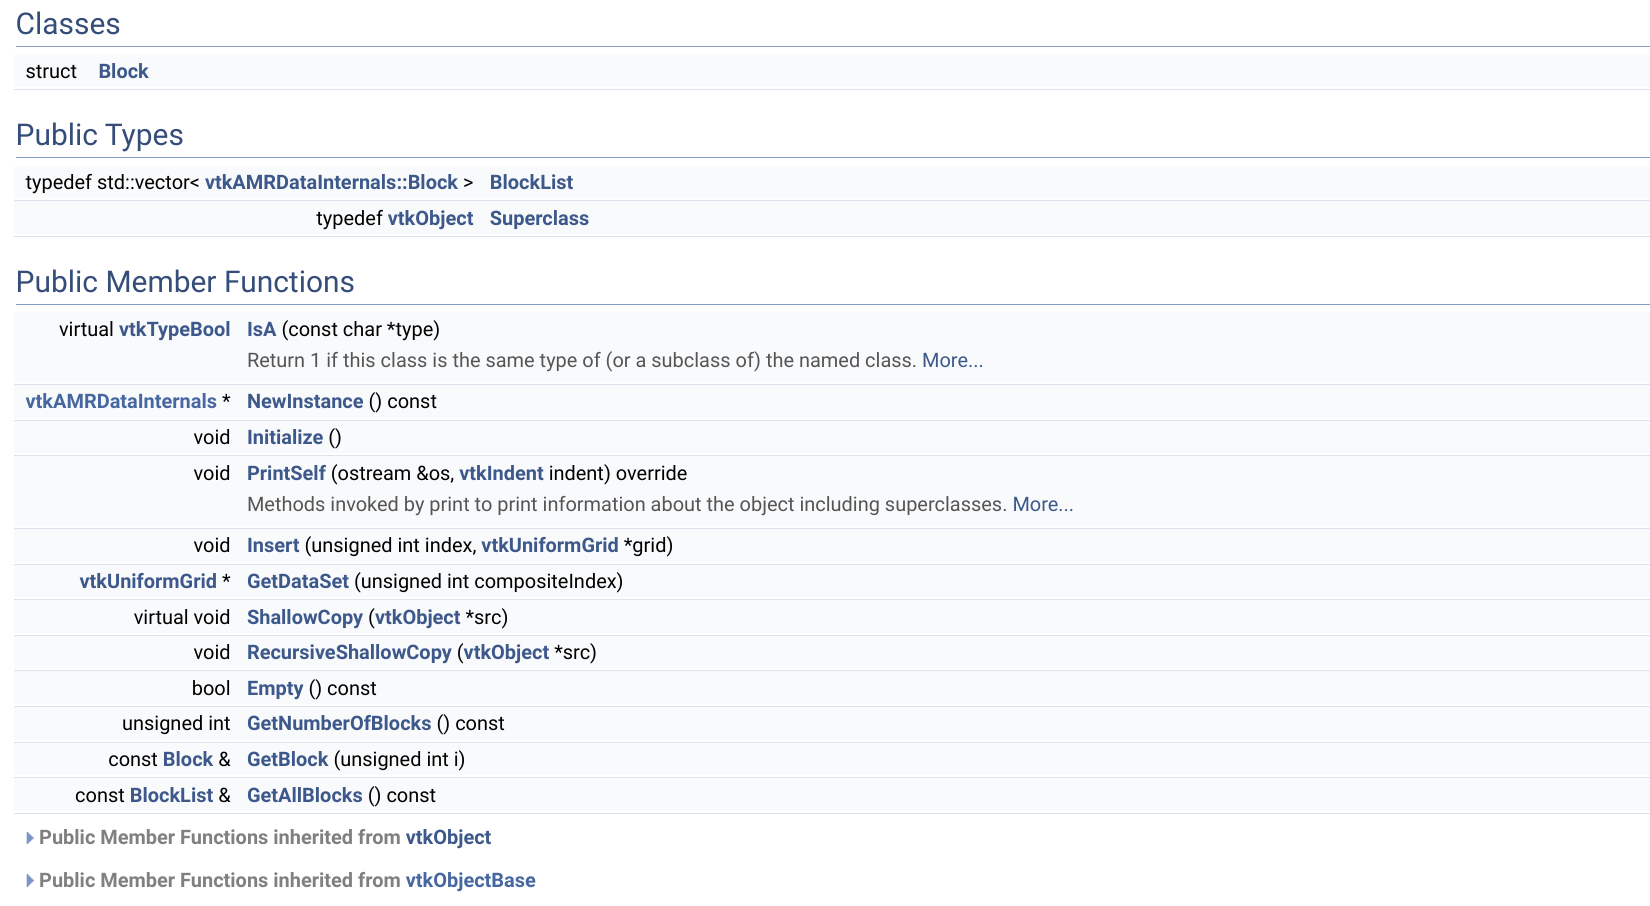
\includegraphics[height=.75\textheight]{./figures/vtk_api.png}

\end{frame}

\begin{frame}
  \frametitle{APIs in the Wild - Python API}
  \vspace{-10pt}

  \href{https://numpy.org/doc/stable/reference/}{NumPy - API Reference}

  \centering
  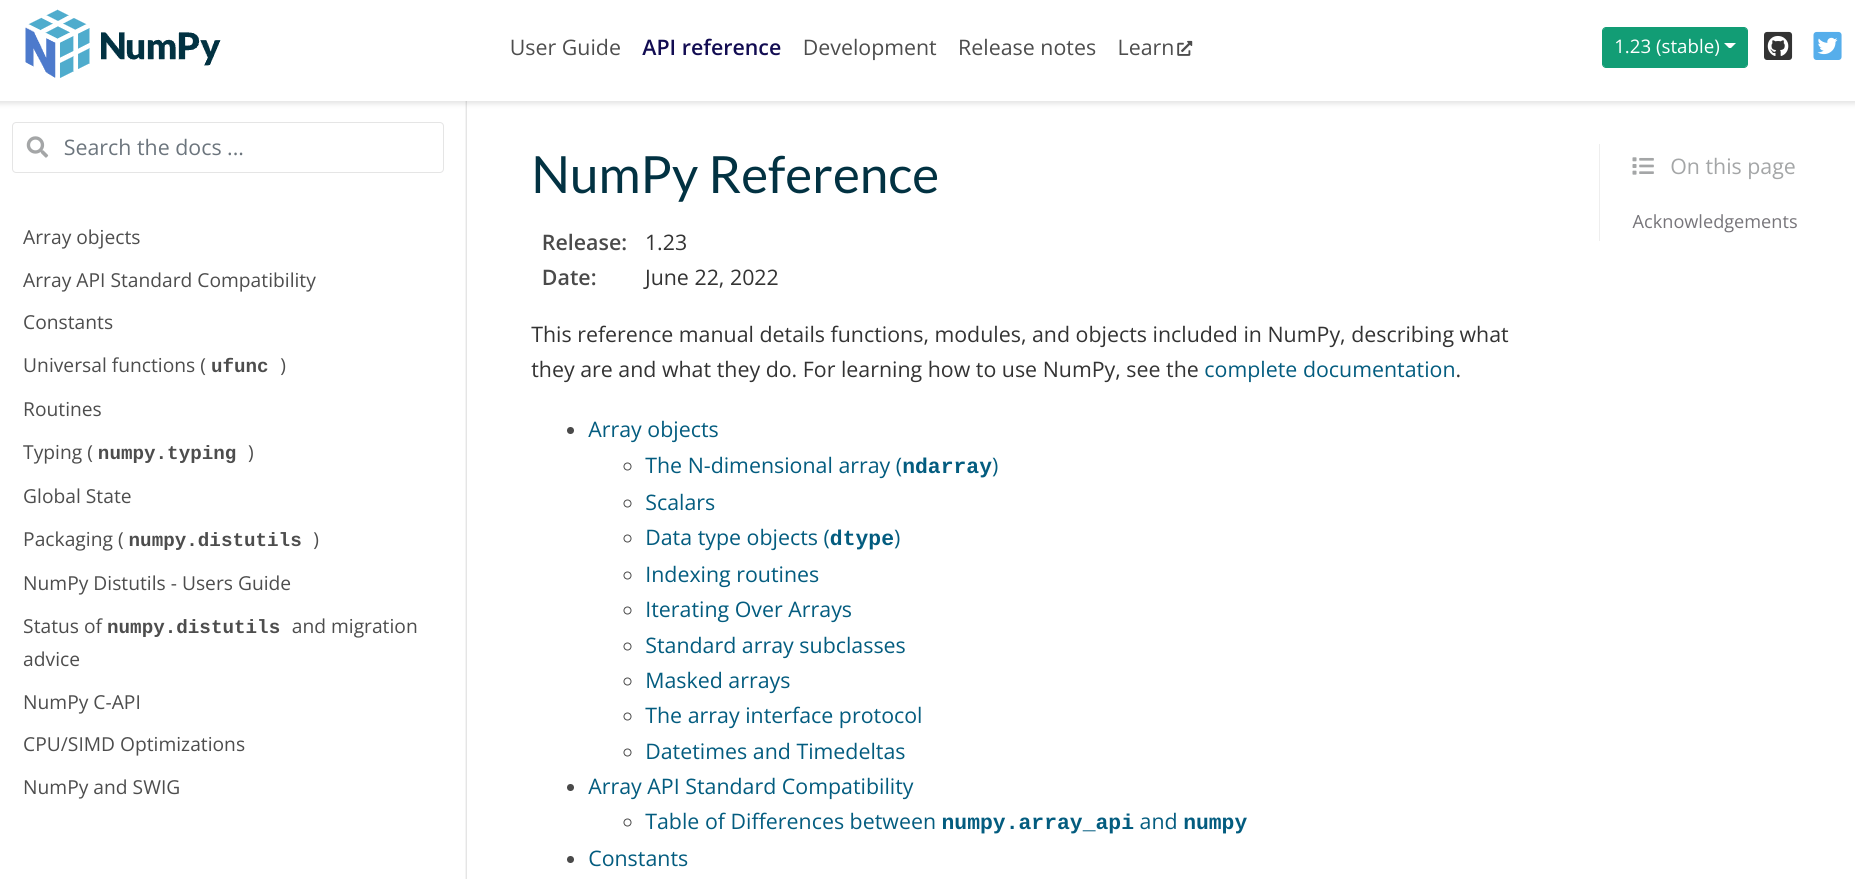
\includegraphics[height=.75\textheight]{./figures/numpy_api.png}

\end{frame}

\subsection{Examples - Network Based}


%%%%%%%%%%%%%%%%%%%%%%%%%%%%%%%%%%%%%%%%%%%%%%%%%%%%%%%%%%%%%%%%%%%%%%%%%%%%%%%
\begin{frame}
  \frametitle{APIs in the Wild - REST API}
  \vspace{-10pt}

  \href{https://onshape-public.github.io/docs/apioverview/}{OnShape - API Reference}

  \centering
  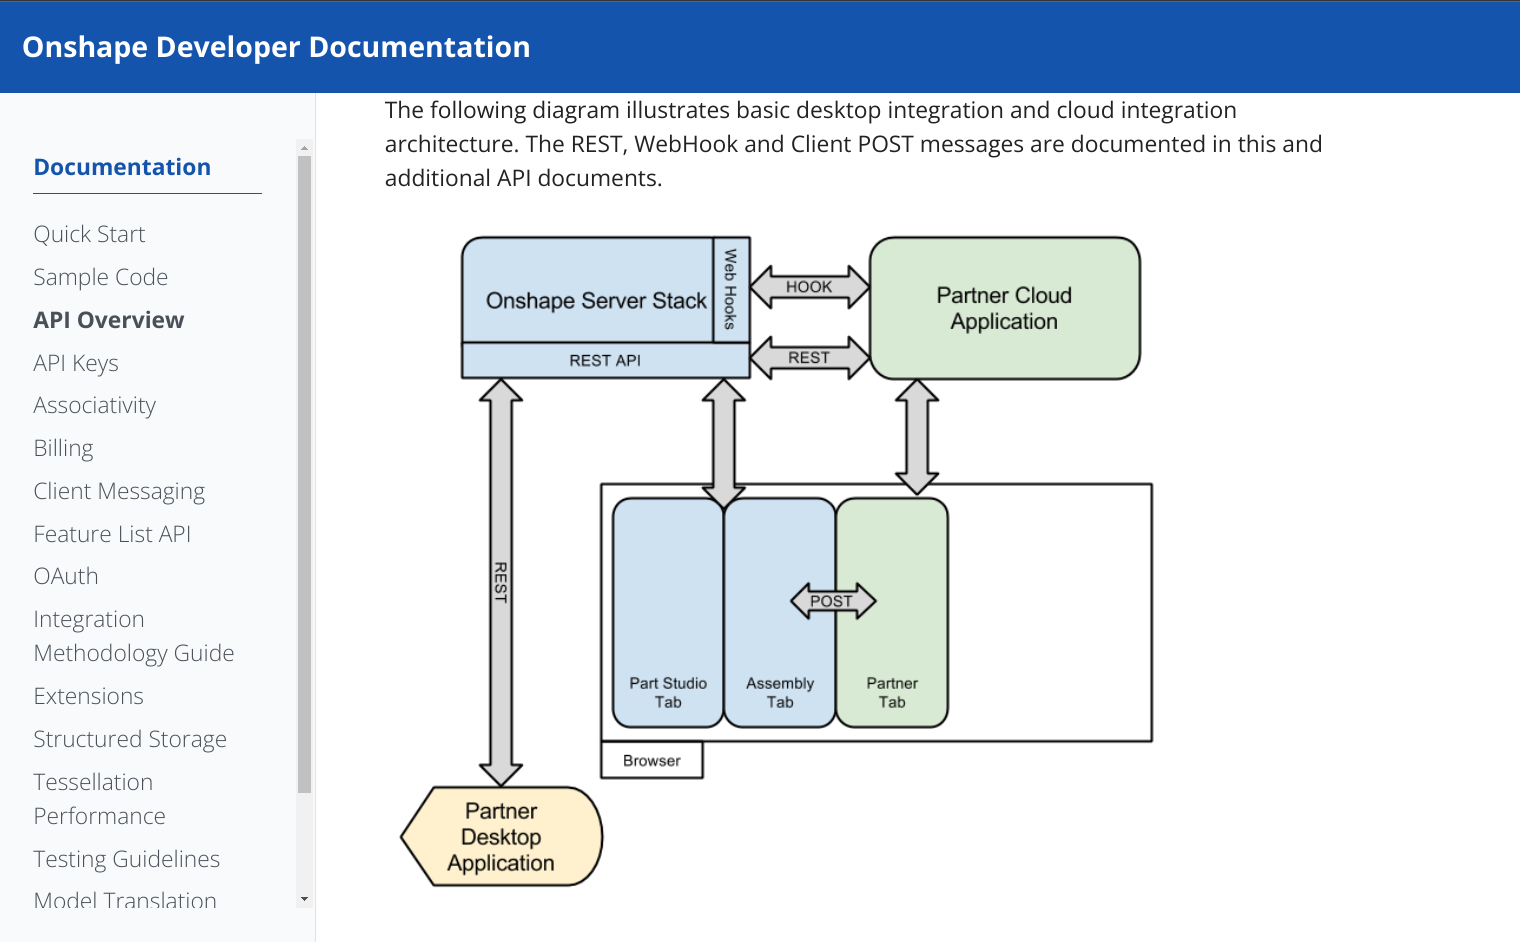
\includegraphics[height=.75\textheight]{./figures/onshape_api.png}

\end{frame}

\begin{frame}
  \frametitle{APIs in the Wild - REST API}
  \vspace{-10pt}

  \href{https://stripe.com/docs/api}{Stripe - API Reference}

  \centering
  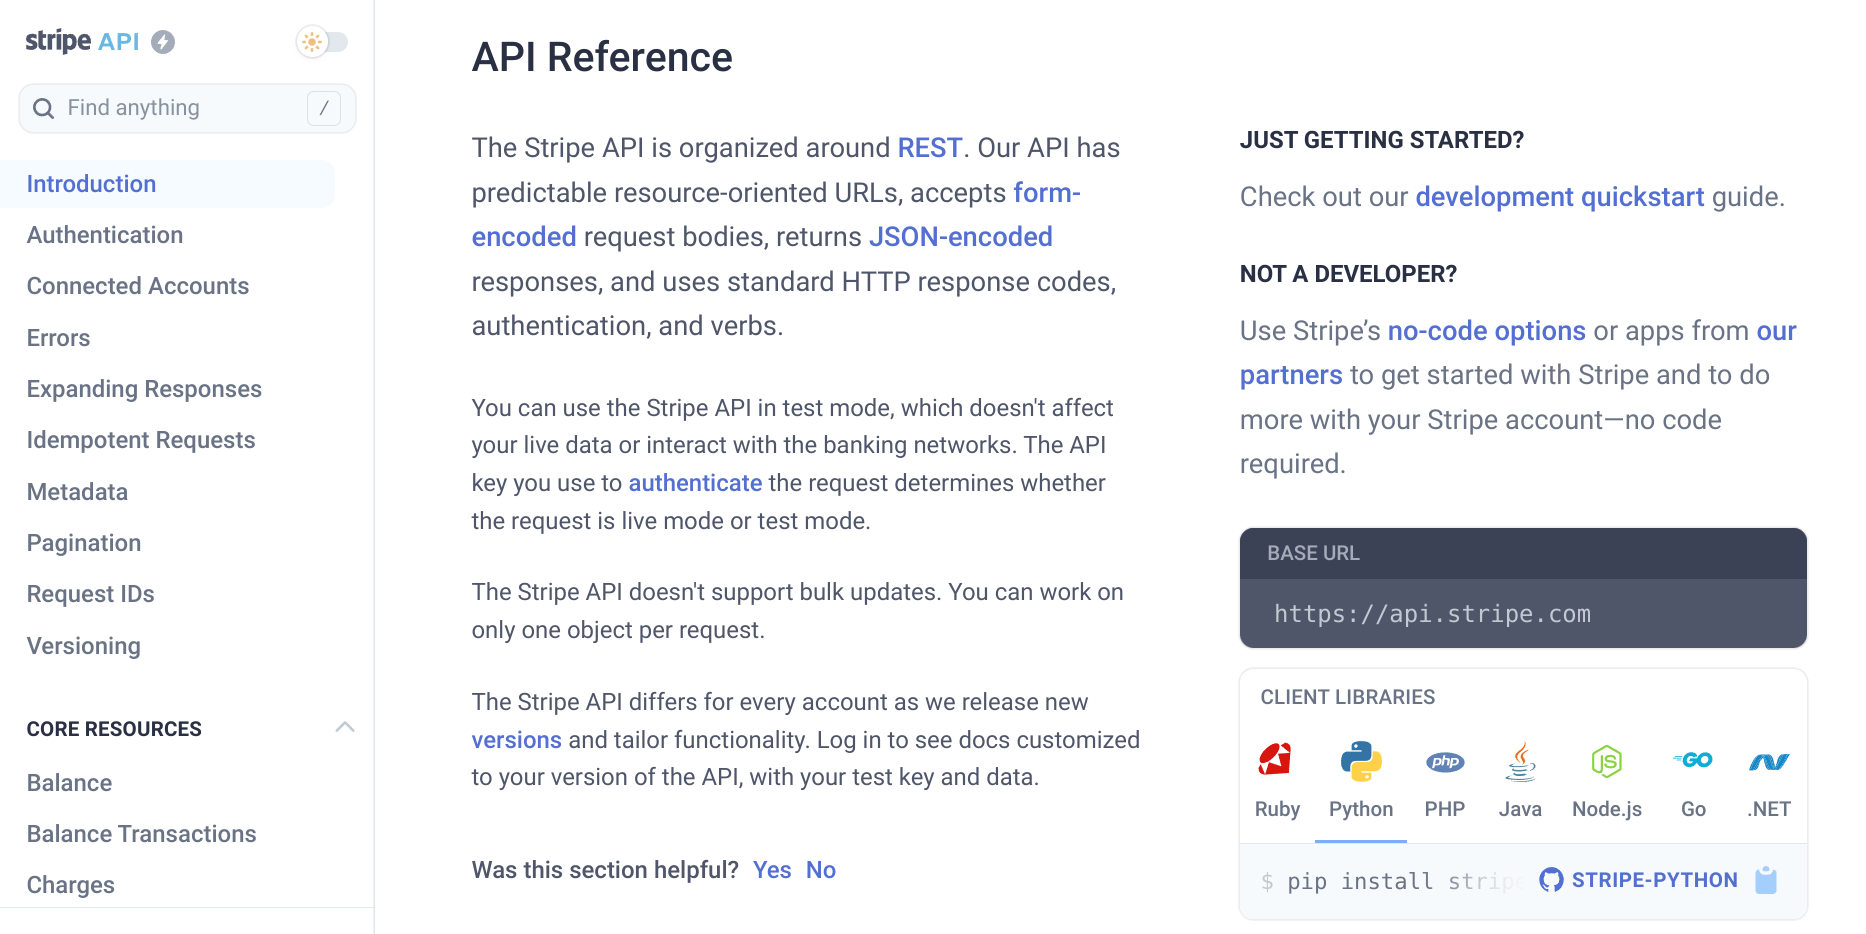
\includegraphics[height=.75\textheight]{./figures/stripe_api.png}

\end{frame}


%%%%%%%%%%%%%%%%%%%%%%%%%%%%%%%%%%%%%%%%%%%%%%%%%%%%%%%%%%%%%%%%%%%%%%%%%%%%%%%
\begin{frame}
  \frametitle{APIs in the Wild - REST API}
  \vspace{-10pt}

  \href{https://kittycad.io/docs/api/}{KittyCAD - API Reference}

  \centering
  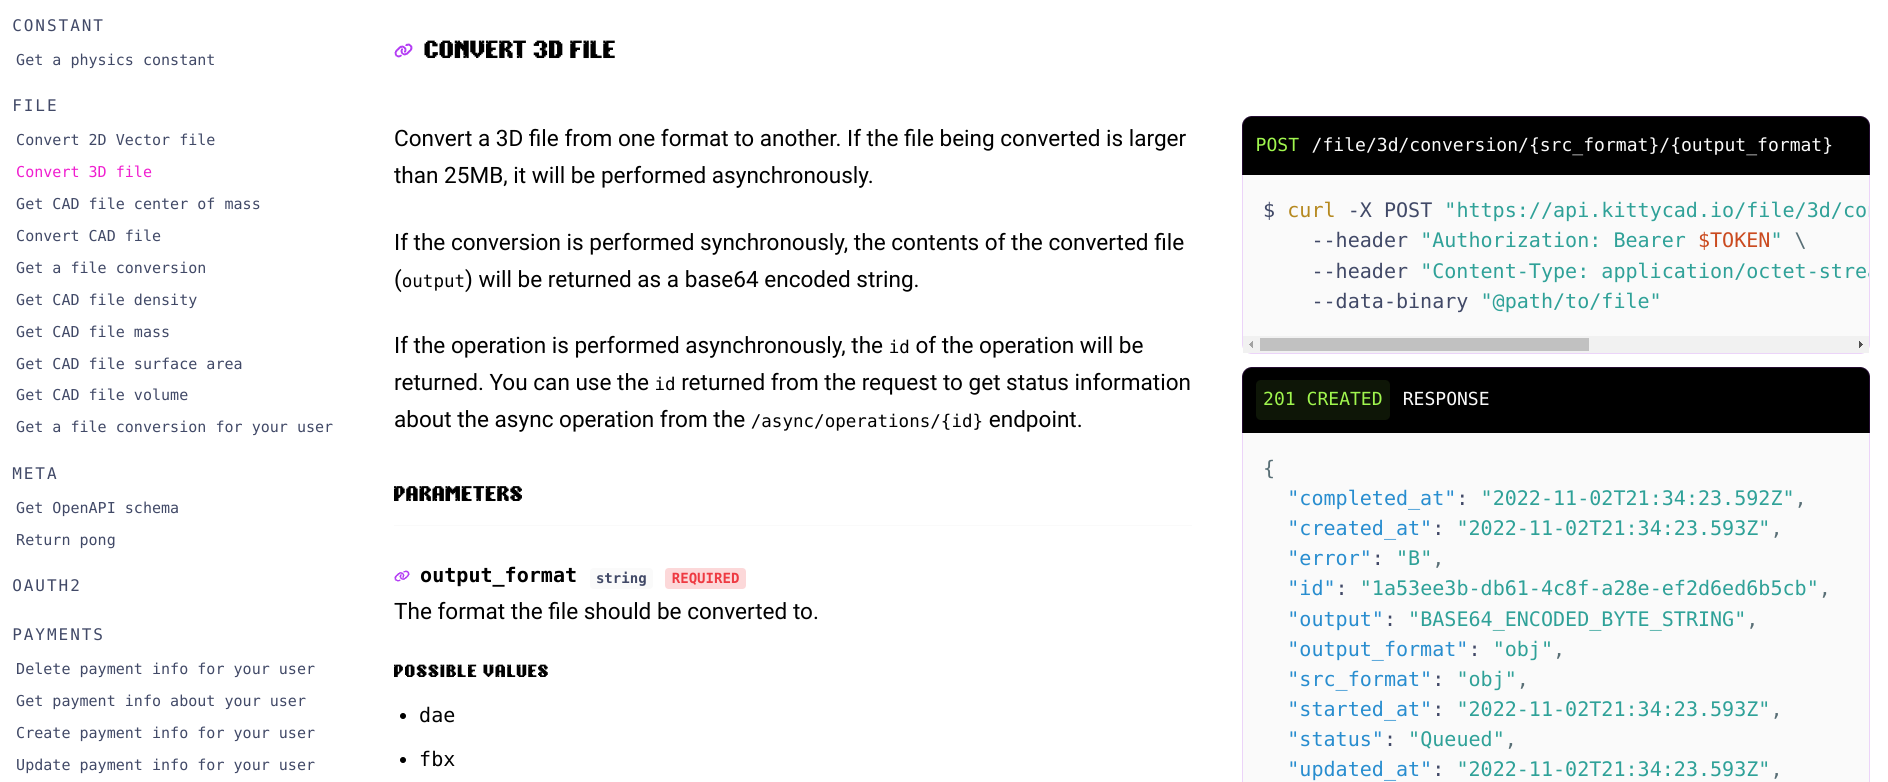
\includegraphics[height=.75\textheight]{./figures/kittycad_api.png}

\end{frame}



%%%%%%%%%%%%%%%%%%%%%%%%%%%%%%%%%%%%%%%%%%%%%%%%%%%%%%%%%%%%%%%%%%%%%%%%%%%%%%%
%% \subsection{Ansys's APIs - C\#}

%% \begin{frame}
%%   \frametitle{Ansys ACT API - C\#}
%%   \inputminted[fontsize=\footnotesize]{csharp}{code/act.cs}
%% \end{frame}


%%%%%%%%%%%%%%%%%%%%%%%%%%%%%%%%%%%%%%%%%%%%%%%%%%%%%%%%%%%%%%%%%%%%%%%%%%%%%%%
\section{Ansys's API - Local and Remote}

\begin{frame}
  \frametitle{Ansys's API - A Holistic Overview}

  To address the need for product automation and low-level access, we need to
  expose three types of APIs:

    \begin{itemize}
      \item Core service/library APIs
      \item Product automation APIs
      \item Remote product APIs
    \end{itemize}

    These three levels of APIs ensure Ansys can enable:

    \begin{itemize}
      \item Inter-product communication without writing to disk
      \item Product customization and automation
      \item Compatibility with cloud infrastructure (e.g. \href{https://www.docker.com/}{Docker})
    \end{itemize}

\end{frame}


%%%%%%%%%%%%%%%%%%%%%%%%%%%%%%%%%%%%%%%%%%%%%%%%%%%%%%%%%%%%%%%%%%%%%%%%%%%%%%%


\begin{frame}
  \frametitle{Ansys's Product APIs - Tech Stack}

  %% Simple pyramid
  \begin{tikzpicture}
    \coordinate (A) at (-4,0) {};
    \coordinate (B) at ( 4,0) {};
    \coordinate (C) at (0,6) {};
    \draw[name path=AC] (A) -- (C);
    \draw[name path=BC] (B) -- (C);
    \foreach \y/\A/\B\C in {
      0/Core Library API/Compiled/ 
\includegraphics[height=.1\textheight]{figures/c-logo.png} 
\includegraphics[height=.1\textheight]{figures/fortran-logo.png},
      2/Product Automation API/Interpreted/ 
\includegraphics[height=.1\textheight]{figures/python-logo.png},
      4/Remote API/Network/ 
\includegraphics[height=.1\textheight]{figures/rest-logo.png} 
\includegraphics[height=.1\textheight]{figures/grpc-logo.png}
    } {
      \path[name path=horiz] (A|-0,\y) -- (B|-0,\y);

      % Level of API
      \draw[name intersections={of=AC and horiz,by=P},
        name intersections={of=BC and horiz,by=Q}] (P) -- (Q)
      node[midway,above] {\A};

      % Language/Architecture
      \draw[name intersections={of=AC and horiz,by=P},
        name intersections={of=BC and horiz,by=Q}] (P) -- (Q)
      node[midway,above,shift={(28ex,0ex)}] {\B};

      % Image
      \draw[name intersections={of=AC and horiz,by=P},
        name intersections={of=BC and horiz,by=Q}] (P) -- (Q)
      node[midway,above,shift={(40ex,0ex)}] {\C};
    }
  \end{tikzpicture}

\end{frame}

%%%%%%%%%%%%%%%%%%%%%%%%%%%%%%%%%%%%%%%%%%%%%%%%%%%%%%%%%%%%%%%%%%%%%%%%%%%%%%%
% low-level part

%%%%%%%%%%%%%%%%%%%%%%%%%%%%%%%%%%%%%%%%%%%%%%%%%%%%%%%%%%%%%%%%%%%%%%%%%%%%%%%
\begin{frame}
  \frametitle{Core Library API - Overview}
  \vspace{-10pt}

  \begin{itemize}
  \item Primarily directed for developers and (rarely) customers wishing to customize at a very low-level.
  \item Core Library API should be exposed in the same language as the library source.
  \item Minimizes code overhead and duplication.
  \end{itemize}

  %% Simple pyramid

  \resizebox{.004\textwidth}{!}{
    \begin{tikzpicture}[overlay]
      \tikzset{shift={(current page.center)},xshift=40cm,yshift=-16cm}
    \coordinate (A) at (-4,0) {};
    \coordinate (B) at ( 4,0) {};
    \coordinate (C) at (0,6) {};
    \draw[name path=AC] (A) -- (C);
    \draw[name path=BC] (B) -- (C);
    \foreach \y/\A in {
      0/Core Library API,
      2/Product Automation API,
      4/Remote API/Network
    } {
      \path[name path=horiz] (A|-0,\y) -- (B|-0,\y);

      % Level of API
      \draw[name intersections={of=AC and horiz,by=P},
        name intersections={of=BC and horiz,by=Q}] (P) -- (Q)
      node[midway,above] ;

      % Language/Architecture
      \draw[name intersections={of=AC and horiz,by=P},
        name intersections={of=BC and horiz,by=Q}] (P) -- (Q)
      node[midway,above,shift={(-28ex,0ex)}] {\huge \A};

    }
  \end{tikzpicture}
  }

\end{frame}

% code snippet
\begin{frame}
  \frametitle{Core Library API - FORTRAN Header}
  \inputminted[fontsize=\footnotesize]{python}{code/fdresu.inc}
\end{frame}


%%%%%%%%%%%%%%%%%%%%%%%%%%%%%%%%%%%%%%%%%%%%%%%%%%%%%%%%%%%%%%%%%%%%%%%%%%%%%%%

\begin{frame}[fragile=singleslide]
  \frametitle{Product Customization and Automation - Product Automation}
  \vspace{-10pt}

  \begin{columns}[T]
    \begin{column}{.5\textwidth}
      \vspace{-5pt}
      \inputminted[fontsize=\footnotesize]{python}{code/pymapdl_example.py}
    \end{column}

    \begin{column}{.5\textwidth}          
      \centering
      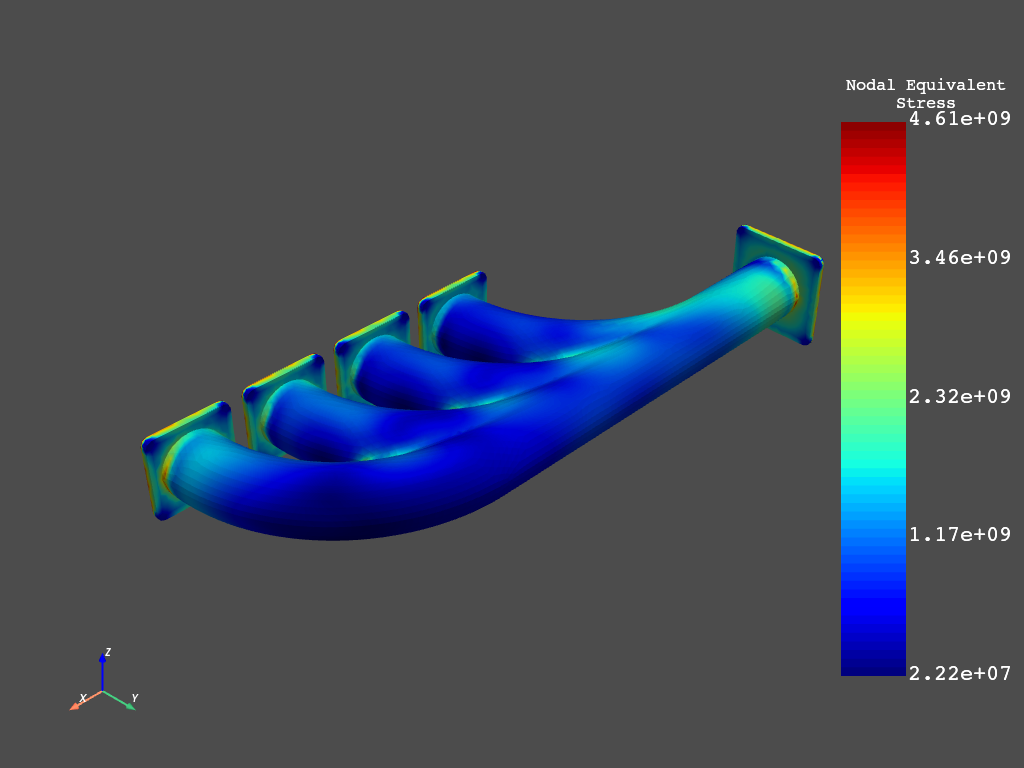
\includegraphics[height=5cm]{figures/sphx_glr_exhaust_manifold_thermal_stress_002.png}
    \end{column}

  \end{columns}
  
\end{frame}


%%%%%%%%%%%%%%%%%%%%%%%%%%%%%%%%%%%%%%%%%%%%%%%%%%%%%%%%%%%%%%%%%%%%%%%%%%%%%%%
\begin{frame}
  \frametitle{Product Customization and Automation - Product Automation}
  \vspace{-10pt}

  \begin{itemize}
  \item Python is one of the top languages used by method developers.
  \item Used as ``glue'' to tie several libraries together as well as perform
    data operations, machine learning, and design optimization.
  \item Wide and deep ecosystem of libraries, frameworks, and tools.
  \end{itemize}

  \centering
  \href{https://www.tiobe.com/tiobe-index/}{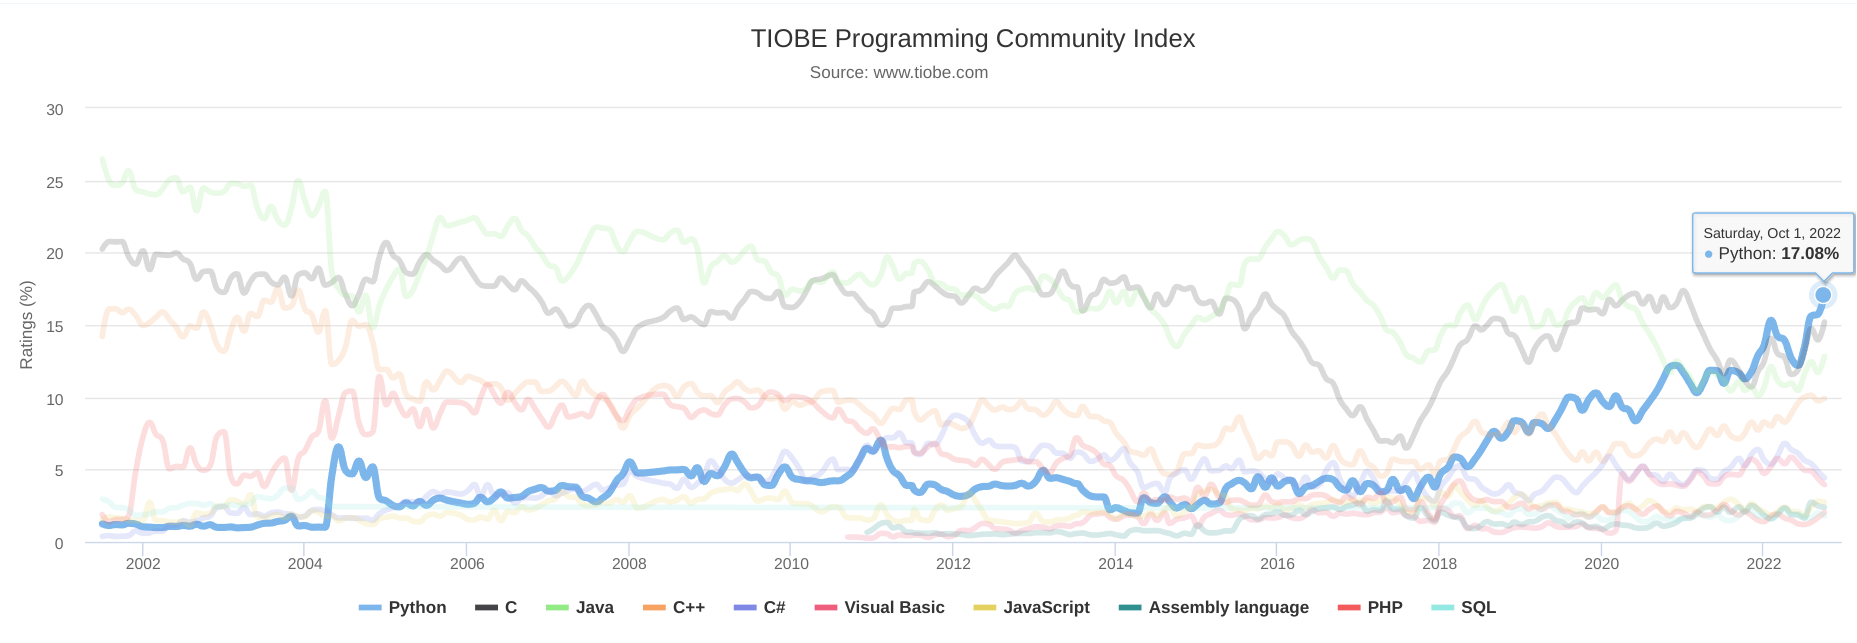
\includegraphics[height=.5\textheight]{./figures/tiobe_index.png}}

\end{frame}



%% %%%%%%%%%%%%%%%%%%%%%%%%%%%%%%%%%%%%%%%%%%%%%%%%%%%%%%%%%%%%%%%%%%%%%%%%%%%%%%%
%% \subsection{End Slide}
%% \begin{frame}[fragile=singleslide]
%%   \frametitle{End Slide}

%%   The end slide can be created with:
%%   \vspace{\baselineskip}

%%   \verb|\lastframe|
%%   \vspace{\baselineskip}

%%   The end slide follows.

%% \end{frame}

%% \lastframe{}

%% %%%%%%%%%%%%%%%%%%%%%%%%%%%%%%%%%%%%%%%%%%%%%%%%%%%%%%%%%%%%%%%%%%%%%%%%%%%%%%%
%% \section{LaTeX Beamer Features}

%% \begin{frame}
%%   \frametitle{LaTeX Beamer Features}
%%   \tableofcontents[currentsection]
%%   \vspace{200pt}  %% force top tight
%% \end{frame}

%% \begin{frame}[fragile=singleslide]
%%   \frametitle{LaTeX Beamer Features}

%%   The Beamer document class contains a variety of features to simplify creating
%%   presentations within LaTeX. This includes:

%%   \begin{itemize}
%%     \item{Title Page}
%%     \item{Table of Contents}
%%     \item{Blocks}
%%   \end{itemize}

%%   For more details, see
%%   \href{https://www.overleaf.com/learn/latex/Beamer}{Overleaf - Beamer}.

%% \end{frame}

%% %%%%%%%%%%%%%%%%%%%%%%%%%%%%%%%%%%%%%%%%%%%%%%%%%%%%%%%%%%%%%%%%%%%%%%%%%%%%%%%
%% \subsection{Title Slide}
%% \begin{frame}[fragile=singleslide]
%%   \frametitle{Title Slide}

%%   The title slide uses the \verb|\titleframe{}| command preceded by commands
%%   containing metadata of the presentation.

%%   \begin{lstlisting}[basicstyle=\footnotesize\ttfamily]

%% \title{Title}
%% \subtitle{Subtitle (optional)}
%% \author{First Middle Last}
%% \date{\today}

%%   \end{lstlisting}

%% \end{frame}

%% %%%%%%%%%%%%%%%%%%%%%%%%%%%%%%%%%%%%%%%%%%%%%%%%%%%%%%%%%%%%%%%%%%%%%%%%%%%%%%%
%% \subsection{Table of Contents}
%% \begin{frame}[fragile=singleslide]
%%   \frametitle{Title Slide}

%%   You can auto-generate a table of contents using the \verb|\tableofcontents|
%%   command. For example:

%%   \begin{lstlisting}[basicstyle=\footnotesize\ttfamily]
%% \begin{frame}{Table of Contents}
%%   \tableofcontents
%%   \vspace{200pt}  %% force top tight  
%% \end{frame}
%%   \end{lstlisting}

%%   This table of contents will be built off of the standard \verb|\section| and
%%   \verb|\subsection| used to organize your presentation. These should precede
%%   key slides right before \verb|\begin{frame}|.

%%   \begin{lstlisting}[basicstyle=\footnotesize\ttfamily]
%% \section{Problem statement}
%% \section{Existing results}
%%     \subsection{Method 1}
%%     \subsection{Method 2}
%% \section{Comparative study}
%%   \end{lstlisting}

%% \end{frame}

%% %%%%%%%%%%%%%%%%%%%%%%%%%%%%%%%%%%%%%%%%%%%%%%%%%%%%%%%%%%%%%%%%%%%%%%%%%%%%%%%
%% \subsection{Blocks}
%% \begin{frame}
%%   \frametitle{Blocks}

%%   Blocks can be used to highlight important points within a presentation.

%%   \begin{block}{Default Block}
%%     Block text.
%%   \end{block}

%%   \begin{alertblock}{Alert Block}
%%     Block text in an alert block.
%%   \end{alertblock}

%%   \begin{examples}
%%     Block text in Ansys Gold block.
%%   \end{examples}

%% \end{frame}


%% %%%%%%%%%%%%%%%%%%%%%%%%%%%%%%%%%%%%%%%%%%%%%%%%%%%%%%%%%%%%%%%%%%%%%%%%%%%%%%%
%% \section{Content}

%% \begin{frame}
%%   \frametitle{Content}
%%   \tableofcontents[currentsection]
%%   \vspace{200pt}  %% force top tight
%% \end{frame}


%% \begin{frame}
%%   \frametitle{Content}
%%   Content in a Beamer presentation can come in a variety of forms, including:

%%   \begin{itemize}
%%     \item{Figures}
%%     \item{Flowcharts}
%%     \item{Code}
%%   \end{itemize}

%%   The following slides provide several examples for how you can include content
%%   in a LaTeX presentation.

%% \end{frame}

%% %%%%%%%%%%%%%%%%%%%%%%%%%%%%%%%%%%%%%%%%%%%%%%%%%%%%%%%%%%%%%%%%%%%%%%%%%%%%%%%
%% \subsection{Figures}
%% \begin{frame}
%%   \frametitle{Figures - Full Slide}
%%   \vspace{-10pt}

%%   Figures can be made to take up most of the slide:

%%   \centering
%%   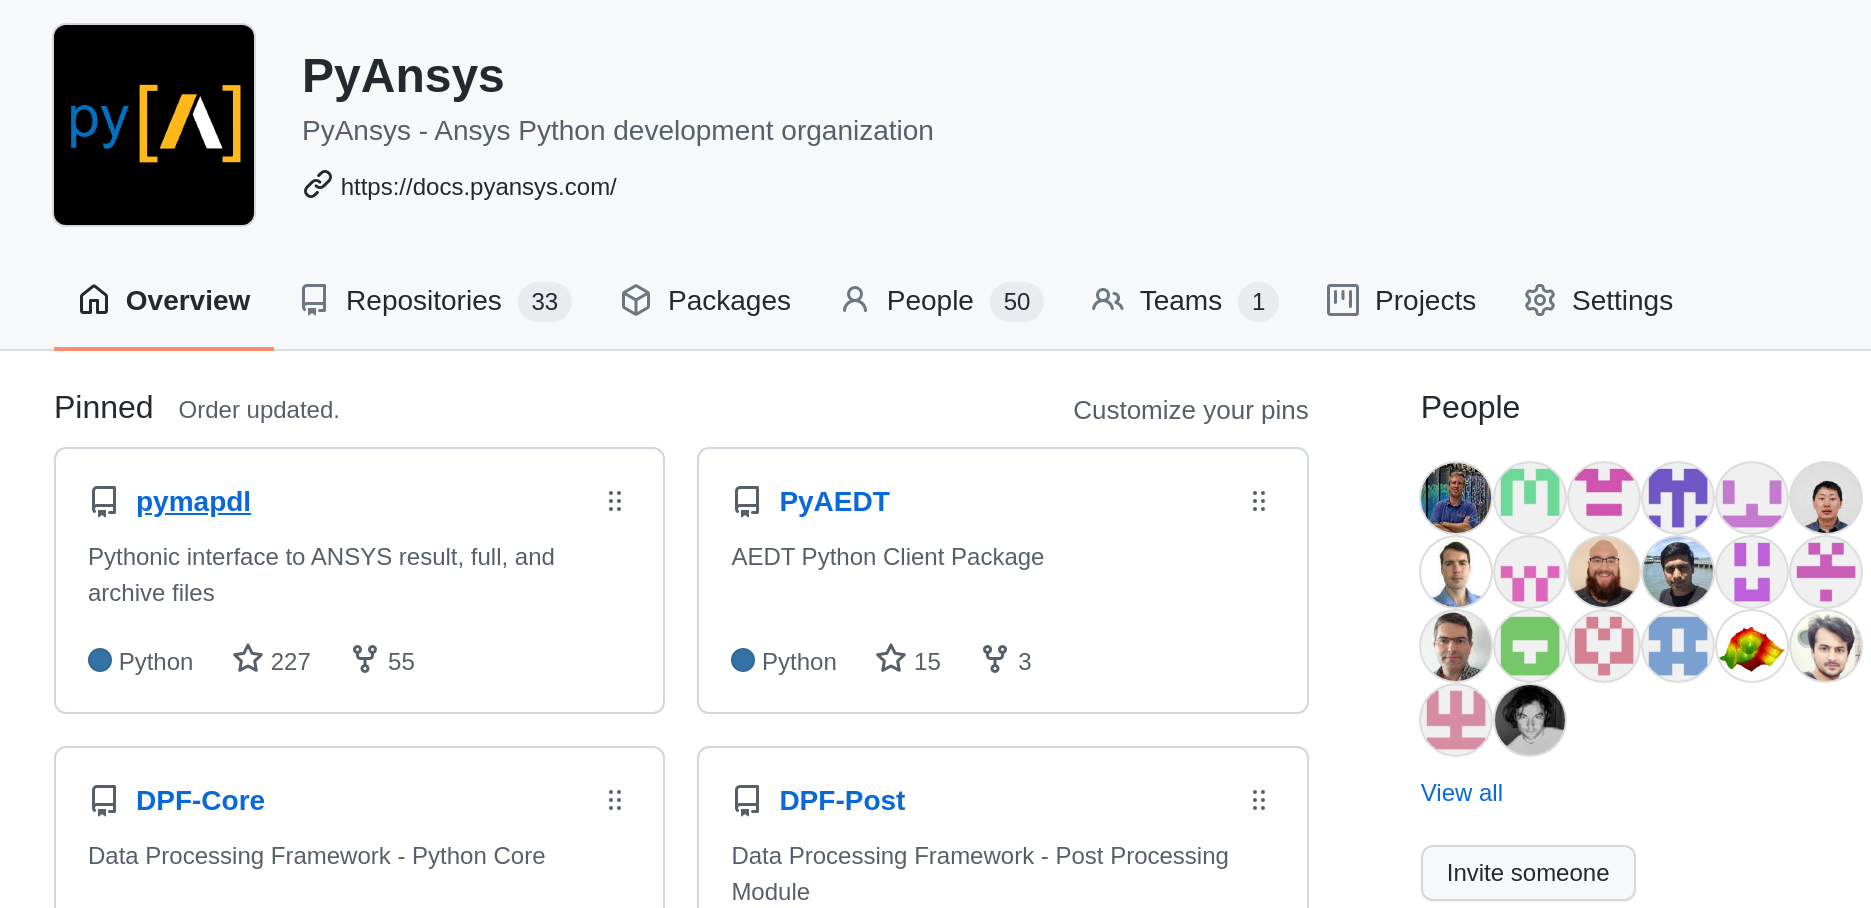
\includegraphics[height=.75\textheight]{./figures/github.png}

%% \end{frame}


%% %%%%%%%%%%%%%%%%%%%%%%%%%%%%%%%%%%%%%%%%%%%%%%%%%%%%%%%%%%%%%%%%%%%%%%%%%%%%%%%
%% \begin{frame}[fragile=singleslide]
%%   \frametitle{Figures - Using Tabular}
%%   \vspace{-10pt}

%%   Figures can also be made to fit alongside text content using either tables or
%%   columns. Here we demonstrate using tables with the figure on the left.

%%   \vspace{6pt}

%%   \begin{tabular}{cl}  
%%     \begin{tabular}{c}
%%       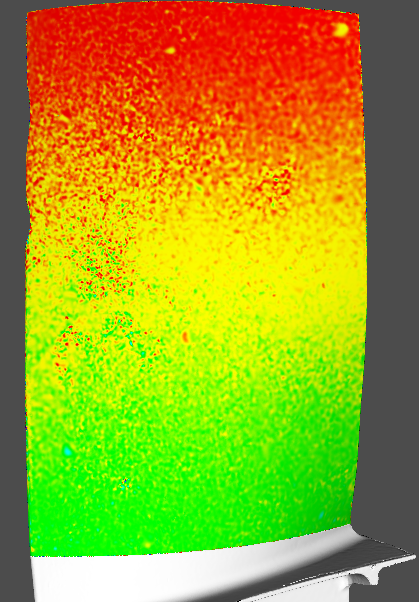
\includegraphics[height=5cm, width=3.5cm]{figures/blade_accuracy.png}
%%     \end{tabular}
%%     & \begin{tabular}{r}
%%         \parbox{0.7\linewidth}{
%%             \begin{itemize}
%%             \item{Item A}
%%             \item{Item B}
%%             \item{Item C}
%%             \end{itemize}
%%         }
%%       \end{tabular}  \\
%% \end{tabular}

%% \end{frame}


%% %%%%%%%%%%%%%%%%%%%%%%%%%%%%%%%%%%%%%%%%%%%%%%%%%%%%%%%%%%%%%%%%%%%%%%%%%%%%%%%
%% \begin{frame}[fragile=singleslide]
%%   \frametitle{Figures - Using Columns}
%%   \vspace{-10pt}

%%   Here we demonstrate showing a figure using two columns with code on the left
%%   and the figure on the right.

%%   \hrulefill{}

%%   \begin{columns}[T]
%%     \begin{column}{.5\textwidth}
%%       \vspace{-5pt}
%%       \inputminted[fontsize=\footnotesize]{python}{code/sample_mpl.py}
%%     \end{column}

%%     \begin{column}{.5\textwidth}          
%%       %% \begin{figure}
%%       \centering
%%       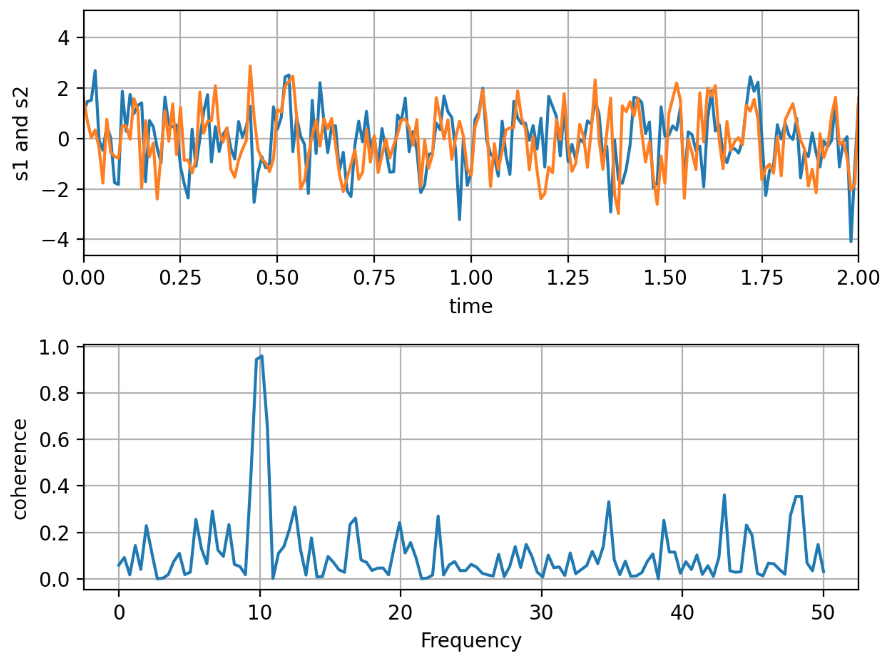
\includegraphics[height=5cm]{figures/sample_mpl.png}
%%       %% \end{figure}
%%     \end{column}

%%   \end{columns}

%% \end{frame}


%% %%%%%%%%%%%%%%%%%%%%%%%%%%%%%%%%%%%%%%%%%%%%%%%%%%%%%%%%%%%%%%%%%%%%%%%%%%%%%%%
%% \subsection{Flowchart}
%% \begin{frame}
%%   \frametitle{Example Flowchart}
%%   \vspace{-10pt}

%%     \begin{columns}[T]
%%         \begin{column}{.6\textwidth}
%%           \begin{itemize}
%%             \item This is a two column slide with a sample flowchart on the right.
%%             \item This flowchart uses the edges package.
%%             \item This two column format is helpful when including figures and
%%               text in the same page.
%%           \end{itemize}
%%         \end{column}


%%         \begin{column}{.4\textwidth}          
%%           \begin{figure}
%%             \centering
%%             \begin{forest}
%%               for tree={
%%                 draw,
%%                 align=center
%%               },
%%               forked edges,
%%               [Front-end\\ (e.g. Python{,} JS{,} or C++),
%%                 [Auto-generated code
%%                   [gRPC Process
%%                     [Application or Service, fill=bleudefrance]
%%                   ]
%%                 ]
%%               ]
%%             \end{forest}
%%           \end{figure}
%%         \end{column}

%%     \end{columns}

%% \end{frame}


%%%%%%%%%%%%%%%%%%%%%%%%%%%%%%%%%%%%%%%%%%%%%%%%%%%%%%%%%%%%%%%%%%%%%%%%%%%%%%%
% End of presentation

\lastframe{}

\end{document}
